\section{Komponenten die Gesamtanwendung}
\setauthor{Hain Lukas}

\begin{figure}[H]
    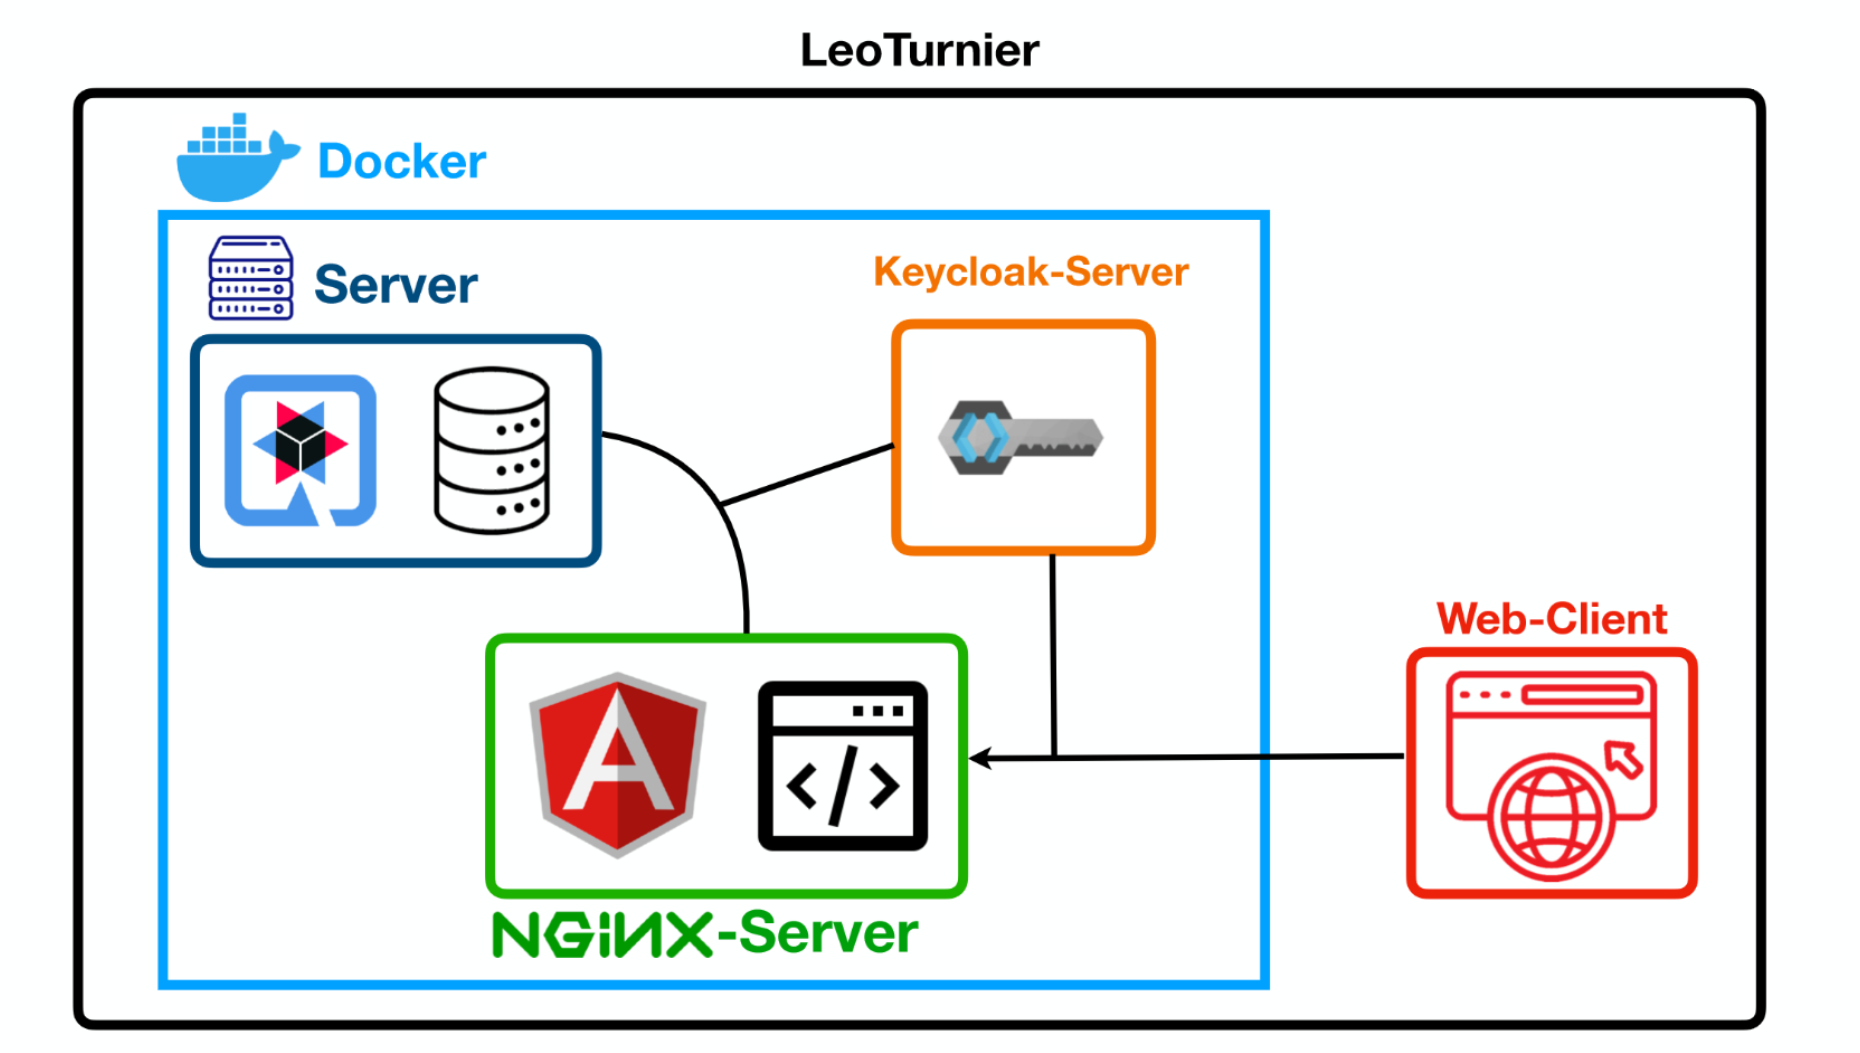
\includegraphics[scale=0.30]{pics/system_architecture_2.png}
    \caption{System Architecture}
\end{figure}

Die Diplomarbeit ist Aufgeteilt in Frontend und Backend. 

\subsection{Backend}
\setauthor{Hain Lukas}

Im Backend befindet sich eine Quarkus Applikation. Sie wurde in Java geschrieben und verwaltet mithilfe von "Hibernate ORM with Panache" Turnierdaten in einer PostgreSQL Datenbank.
Diese Daten werden dem Frontend mithilfe von "RESTEasy" zur Verfügung gestellt. Außerdem greift die Quarkus Applikation mithilfe von "Quarkus OIDC" auf einen KeyCloak Server zu. 
Die Quarkus Applikation sowie die PostgreSQL Datenbank werden in jeweils einem Docker Container ausgeführt.

\subsection{Frontend}
\setauthor{Ecker Benjamin}

Das Frontend besteht aus einer Angular Applikation. Diese wurde in TypeScript als Code-Behind und HTML als Auszeichnungssprache geschrieben. Für ein schönes und konsistentes User Interface
verwendet sie die Library Angular Material. Mithilfe eines KeyCloak Servers wird eine funktionierende Zugriffverwaltung der verschiedenen Benutzer garantiert.
Um diesen richtig benützen zu können wird das KeyCloak-Angular Module von Mauricio Vigolo \cite{sysarch-keycloak-angular-1} verwendet. Sonstige Funktionen, wie etwa Routing und ein HttpClient, werden fast zur Gänze von der Library
Angular Common abdeckt.
Die gesamte Angular Anwendung wird dazu noch auf einen Nginx Server deployed welcher in einem Docker Container ausgeführt wird. 

\subsection{KeyCloak}

Der Keycloak Server ist dafür verantwortlich, die Userdaten zu verwalten, und bestimmte Funktionen der Applikation nur für bestimmte Rollen freizugeben. 
Die Userdaten sind in einer PostgreSQL Datenbank gespeichert. Der keyCloak Server und die Datenbank werden beide jeweils in einem Docker Container ausgeführt.

\section{Verwirklichung der Anforderungen}

TODO

?